\hypertarget{database_8cpp}{}\section{src/database.cpp File Reference}
\label{database_8cpp}\index{src/database.\+cpp@{src/database.\+cpp}}


\hyperlink{classDatabase}{Database} constructor.  


{\ttfamily \#include $<$iostream$>$}\newline
{\ttfamily \#include $<$stdio.\+h$>$}\newline
{\ttfamily \#include \char`\"{}database.\+h\char`\"{}}\newline
{\ttfamily \#include \char`\"{}exception.\+h\char`\"{}}\newline
Include dependency graph for database.\+cpp\+:
\nopagebreak
\begin{figure}[H]
\begin{center}
\leavevmode
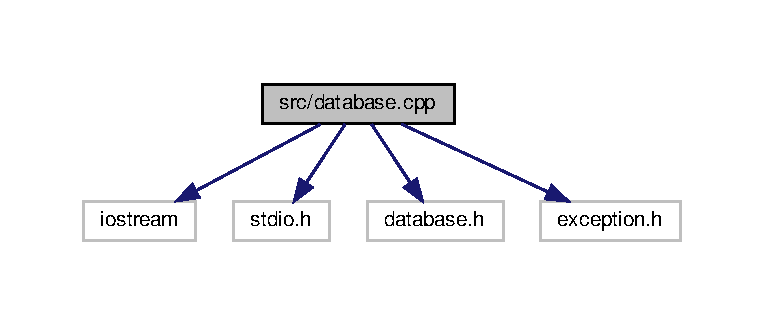
\includegraphics[width=350pt]{database_8cpp__incl}
\end{center}
\end{figure}


\subsection{Detailed Description}
\hyperlink{classDatabase}{Database} constructor. 

Deletes a row from the database.

Returns the database filename.

Creates a new database.

Finds a row in the database.

Writes a row to the database.

Reads a row from the database.

Saves a database.

Loads a database into memory.

\hyperlink{classDatabase}{Database()}

\begin{DoxyAuthor}{Author}
Matthew Boote
\end{DoxyAuthor}

\begin{DoxyParams}[1]{Parameters}
\mbox{\tt in}  & {\em None} & \\
\hline
\mbox{\tt out}  & {\em None} & \\
\hline
\end{DoxyParams}
\begin{DoxyReturn}{Returns}
Boolean None
\end{DoxyReturn}
Load()

\begin{DoxyAuthor}{Author}
Matthew Boote
\end{DoxyAuthor}

\begin{DoxyParams}[1]{Parameters}
\mbox{\tt in}  & {\em std\+::string} & filename\\
\hline
\mbox{\tt out}  & {\em None} & \\
\hline
\end{DoxyParams}
\begin{DoxyReturn}{Returns}
Boolean true or false
\end{DoxyReturn}
Save()

\begin{DoxyAuthor}{Author}
Matthew Boote
\end{DoxyAuthor}

\begin{DoxyParams}[1]{Parameters}
\mbox{\tt in}  & {\em std\+::string} & filename\\
\hline
\end{DoxyParams}
\begin{DoxyReturn}{Returns}
Boolean true or false
\end{DoxyReturn}

\begin{DoxyExceptions}{Exceptions}
{\em Throws} & an error on file I/O error\\
\hline
\end{DoxyExceptions}
Read()

\begin{DoxyAuthor}{Author}
Matthew Boote
\end{DoxyAuthor}
Reads a row of key+values from the database \begin{DoxyVerb}@param[in] std::string key

@param[out] None

@return std::vector<std::string>\end{DoxyVerb}


Write()

\begin{DoxyAuthor}{Author}
Matthew Boote
\end{DoxyAuthor}
Writes a row of key+values to the database \begin{DoxyVerb}@param[in] std::string key,std::vector<std::string> valuevector

@param[out] None

@return std::vector<std::string>\end{DoxyVerb}


Find()

\begin{DoxyAuthor}{Author}
Matthew Boote
\end{DoxyAuthor}
Finds the next row in turn in the database \begin{DoxyVerb}@param[in] None

@param[out] None

@return std::vector<std::string>\end{DoxyVerb}


New()

\begin{DoxyAuthor}{Author}
Matthew Boote
\end{DoxyAuthor}
Creates a database object and corresponding file. \begin{DoxyVerb}@param[in] std::string filename

@param[out] None

@return boolean true or false

@throw Throws on I/O error\end{DoxyVerb}


Get\+File\+Name()

\begin{DoxyAuthor}{Author}
Matthew Boote
\end{DoxyAuthor}

\begin{DoxyParams}[1]{Parameters}
\mbox{\tt in}  & {\em None} & \\
\hline
\mbox{\tt out}  & {\em None} & \\
\hline
\end{DoxyParams}
\begin{DoxyReturn}{Returns}
std\+::string database\+\_\+filename
\end{DoxyReturn}
Delete()

\begin{DoxyAuthor}{Author}
Matthew Boote
\end{DoxyAuthor}
Deletes a row associated with a key \begin{DoxyVerb}@param[in] None

@param[out] None

@return boolean true or false\end{DoxyVerb}
